\documentclass[12pt]{report}

\usepackage[utf8]{inputenc}
%\usepackage[T1]{fontenc}
%\usepackage[français]{babel}
\usepackage{color}
\usepackage[OT1]{fontenc}
\usepackage{lipsum}
\usepackage{graphicx}
\usepackage{geometry}

\begin{document}
	 Nous avons utilisez le logiciel de modélisation open-source {\tt Modelio} le long de la phase de conception.
		
		\begin{center}
			
\includegraphics[scale=1, width=0.56\textwidth, height=4cm]{modelio}
			\label{modelio}
		\end{center}
	
	Nous avons préféré l'éditeur de te
	 Visual-Studio-Code 1.28 Un éditeur de texte avancé
		\begin{center}
			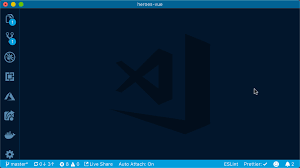
\includegraphics[scale=1, width=0.5\textwidth, height=5cm]{vscode}
			\label{vscode}
		\end{center}
		Flask 1.0:  Un \textit{mini-framework} open-source de développement web en Python
		
		\begin{center}
			
\includegraphics[scale=1, width=0.5\textwidth, height=4cm]{flask}
			\label{flask}
		\end{center}
		 Jinja2: Un moteur de template
		\begin{center}
			
\includegraphics[scale=1, width=0.5\textwidth, height=4cm]{jinja}
			\label{jinja}
		\end{center}
		
		Mongo-DB: Un système de gestion de base de données orienté document open-source developpé en {\tt C++}
		\begin{center}
			
\includegraphics[scale=1, width=0.5\textwidth, height=4cm]{mongo}
			\label{mongo}
		\end{center}
		
		
\end{document}
